% Junbiao Huang's mathematical control-journal report style.
\documentclass[lang=en,11pt,a4paper,bibend=bibtex]{elegantpaper}
\usepackage{xeCJK}
\setCJKmainfont{FandolSong-Regular.otf}
\setCJKsansfont{FandolSong-Regular.otf}
\setCJKmonofont{FandolSong-Regular.otf}
\usepackage{tikz,pgfplots,tabularx,titlesec,fancyhdr}
\usetikzlibrary{arrows.meta,positioning,calc}
\pgfplotsset{compat=1.18}
\geometry{left=23mm,right=23mm,top=21mm,bottom=22mm,headheight=15pt,headsep=7mm}
\linespread{1.10}
\setlength{\parindent}{0pt}
\setlength{\parskip}{5pt}
\setlength{\emergencystretch}{2em}
\definecolor{accent}{HTML}{234D64}
\definecolor{muted}{HTML}{59646C}
\definecolor{light}{HTML}{F0F4F6}
\hypersetup{colorlinks=true,linkcolor=accent,urlcolor=accent}
\titleformat{\section}{\Large\sffamily\bfseries\color{accent}}{\thesection}{0.6em}{}
\titleformat{\subsection}{\normalsize\sffamily\bfseries}{\thesubsection}{0.6em}{}
\titlespacing*{\section}{0pt}{9pt}{8pt}
\titlespacing*{\subsection}{0pt}{8pt}{3pt}
\pagestyle{fancy}
\fancyhf{}
\fancyhead[L]{\small\sffamily\color{muted}EXPERIMENT 2\enspace /\enspace ROBOMASTER EP}
\fancyhead[R]{\small\sffamily\color{muted}\studentname}
\fancyfoot[L]{\small\sffamily\color{muted}\studentid\quad\textbullet\quad Individual laboratory report}
\fancyfoot[R]{\small\sffamily\thepage}
\renewcommand{\headrulewidth}{0.3pt}
\renewcommand{\footrulewidth}{0pt}
\captionsetup{font=small,labelfont=bf,labelsep=period,skip=5pt,hypcap=false}
\renewcommand{\arraystretch}{1.18}
\newcolumntype{Y}{>{\raggedright\arraybackslash}X}
\newcommand{\code}[1]{{\small\nolinkurl{#1}}}
\newcommand{\source}[1]{{\small\color{muted}Source: #1}\par}
\newcommand{\reportnote}[1]{\par\smallskip\noindent\colorbox{light}{\parbox{\dimexpr\linewidth-2\fboxsep}{\small #1}}\par\smallskip}
\newcommand{\reporttitle}[1]{\vspace*{2mm}{\small\sffamily\bfseries\color{accent}FIXED-POINT PICK-AND-PLACE}\par\vspace{2mm}{\LARGE\sffamily\bfseries #1\par}\vspace{3mm}{\large\studentname\enspace\studentcn}\par{\small Student ID: \studentid\quad |\quad Individual report}\par\vspace{3mm}\hrule\vspace{3mm}}
\tikzset{box/.style={draw=accent,fill=light,rounded corners=2pt,align=center,font=\small,minimum height=9mm},arr/.style={-{Latex[length=2mm]},thick,draw=accent}}
\newcommand{\teamtable}{%
\par\smallskip
\begingroup\small\renewcommand{\arraystretch}{1.08}
\begin{tabularx}{\linewidth}{@{}>{\raggedright\arraybackslash}p{25mm}>{\raggedright\arraybackslash}p{21mm}Y@{}}\toprule
Member & Work area & Main responsibility \\\midrule
Ning Bo & Simulation & Set up the environment and scene; load models and launch the simulation.\\
Huang Junbiao & Simulation & Work on the motion program and debug grasping, transfer and repeated cycles.\\
Qi Yongyue & Simulation results & Organize logs, analyse results and prepare report material.\\
Bao Lintai & Hardware & SDK communication, task sequence, chassis turn/return and exception handling; joint trials.\\
Xue Yutong & Hardware & Pick/release waypoints, approach/lift heights, gripper adjustment and retention checks; joint trials.\\\bottomrule
\end{tabularx}\par\endgroup}
\newcommand{\commonrequirements}{%
\section{Experiment requirements and individual scope}
The experiment develops a fixed-point grasping task without visual localization: home, approach A, descend, grip, lift, transfer to B, release and return. The course requires a complete simulation launch, state publication, saved trajectories/results/errors, joint and reachability checks, and at least four successful transfers in five consecutive trials. Hardware verification additionally requires supervised low-speed operation, safe failure handling and individual safety-operation checks [1].

Because of equipment availability, our group used the DJI RoboMaster EP arm and gripper instead of the specified mechArm 270. The simulation uses ROS 2 Humble, Gazebo Fortress and custom kinematics/control on a Jetson Linux system. The physical implementation uses the RoboMaster Python SDK. This is a platform adaptation, not an unchanged ROS 2 hardware backend.
}
\newcommand{\commonlimits}{%
\reportnote{Scope of evidence. Simulation repeats A$\rightarrow$B and verifies home after every cycle; the object is reset only between cycles. Hardware alternates A/B, pauses for human grasp confirmation and returns home after all five cycles. Shared ROS 2 interfaces, parameter-only hardware switching and each member's safety check are not demonstrated by the supplied records.}}
\newcommand{\mainresults}{%
\begin{center}\small
\begin{tabular}{@{}crrrcc@{}}\toprule
Cycle & Error (mm) & Heading ($^\circ$) & Time (s) & Placed & Home \\\midrule
1 & 2.274 & 0.445 & 67.01 & Yes & Yes\\
2 & 5.604 & 0.329 & 59.72 & Yes & Yes\\
3 & 4.192 & 0.404 & 60.92 & Yes & Yes\\
4 & 4.577 & 0.459 & 61.09 & Yes & Yes\\
5 & 5.144 & 0.405 & 61.29 & Yes & Yes\\\bottomrule
\end{tabular}
\end{center}
\source{Recorded simulation run \code{20260913_153855_682865/results.json}; error is horizontal distance from configured B, heading is absolute home-heading error.}}
\newcommand{\hardwareresult}{%
\subsection{Physical validation: team-observed outcome}
The team confirmed that all five hardware transfers succeeded with no observed abnormalities. Cycles 1, 3 and 5 moved A$\rightarrow$B; cycles 2 and 4 moved B$\rightarrow$A. Each lift was followed by a fresh human \code{y} confirmation before rotation; final heading restoration and homing followed cycle 5. This is an observed 5/5 result, not an instrumented precision or timing measurement. No real-hardware position-error, duration or force data are available, and five successes do not establish long-run reliability.}
\newcommand{\githubsection}{%
\clearpage
\section{Shared GitHub repository and commit evidence}
The complete group archive is stored in the
\href{https://github.com/ccx8kg5qpd-debug/robomaster-ep-fixed-point-grasping}
{shared public GitHub repository}. The repository address is
\nolinkurl{github.com/ccx8kg5qpd-debug/robomaster-ep-fixed-point-grasping}.
It contains the simulation and hardware programs, model resources, saved results,
the complete simulation recording and all five individual report sources.

\begin{center}
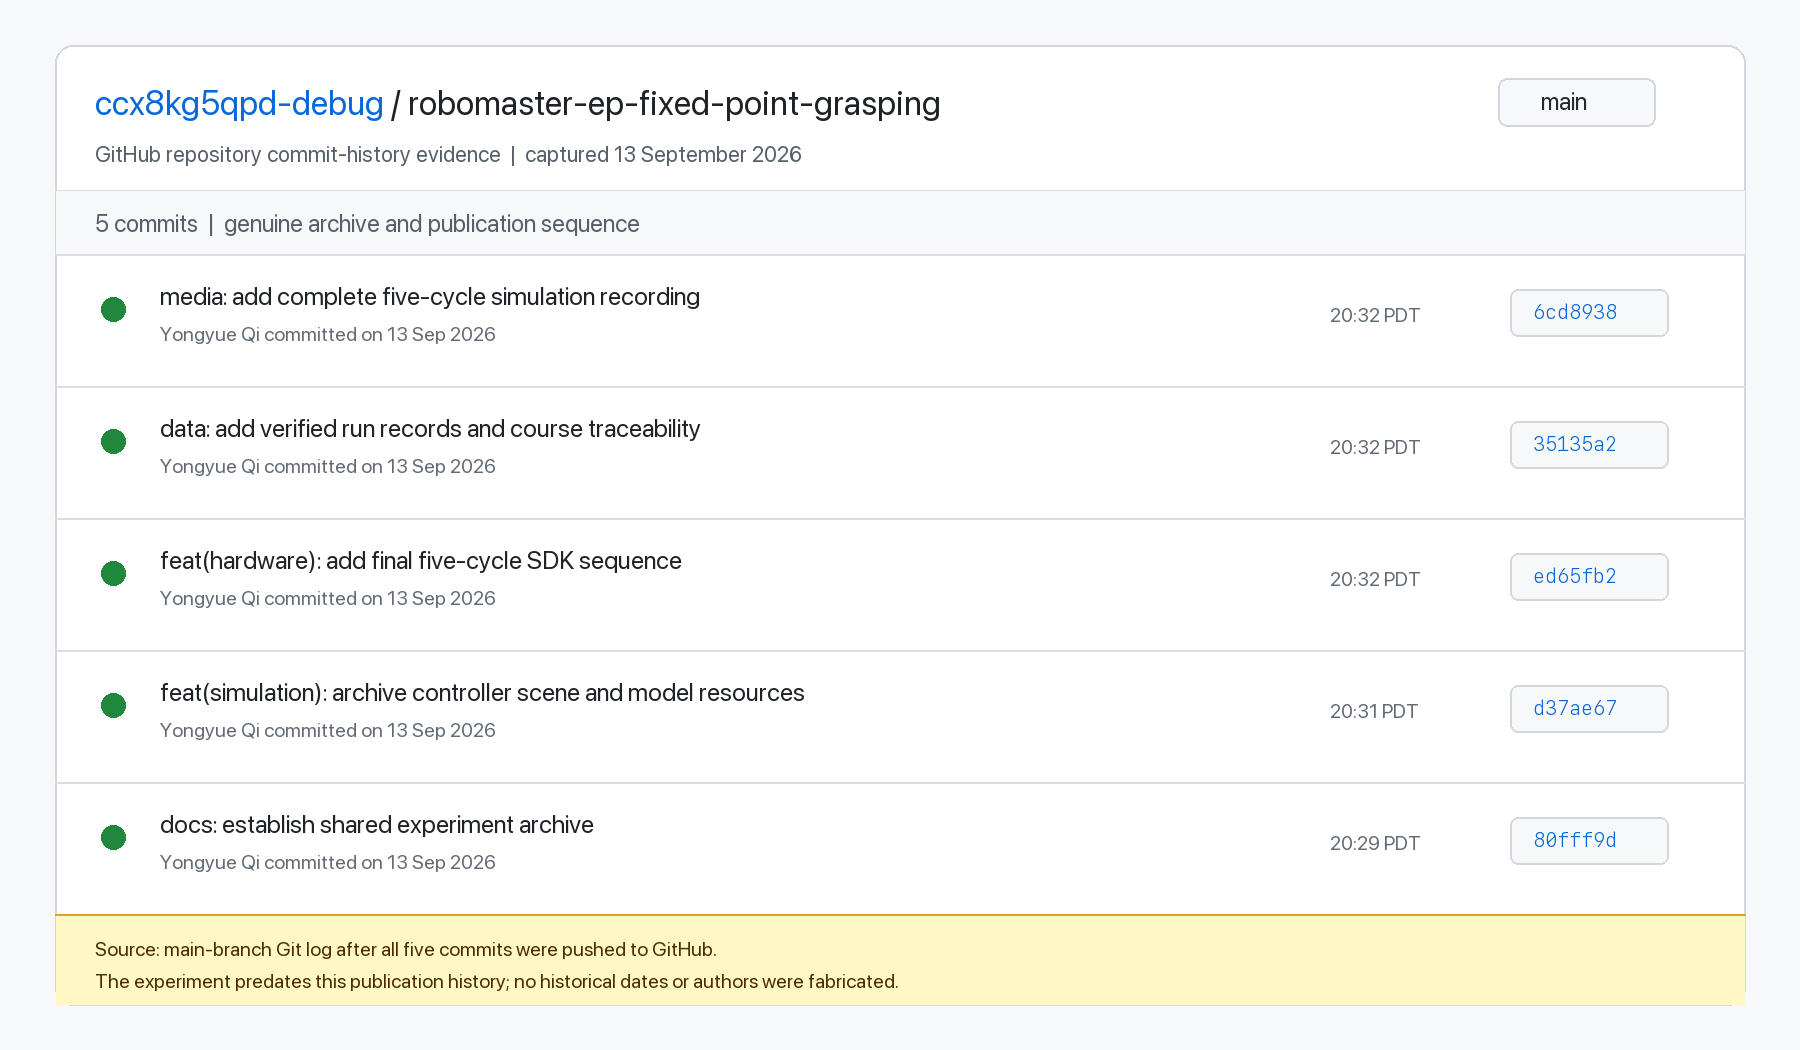
\includegraphics[width=\linewidth]{assets/commit_history_snapshot.png}
\captionof{figure}{Commit-history evidence captured after the first five project
materials commits had been pushed to the shared GitHub repository.}
\end{center}

\reportnote{Traceability note. The experiment was completed before the GitHub
repository was assembled. These genuine commits document the later review,
organization and publication sequence; they are not presented as a fabricated
contemporaneous development history. The screenshot records the five commits
visible at capture time, before this revised report was added.}
}
\newcommand{\referencesblock}{%
\section*{Sources and traceability}
{\footnotesize
[1] Course handout, \emph{Fixed-Point Robotic-Arm Grasping: Simulation Development and Hardware Validation}, S16--S20 / E5; individual-report assignment requirements.\par
[2] Shared team repository, \href{https://github.com/ccx8kg5qpd-debug/robomaster-ep-fixed-point-grasping}{robomaster-ep-fixed-point-grasping}, assembled 13 September 2026: simulation source/configuration, \code{real_v2_five_cycles_manual.py}, saved logs and reports. Primary numerical record: \code{20260913_153855_682865}.\par
[3] Team conversation fact-check materials, 13 September 2026, for development history; subsequent team confirmation for the completed five-cycle hardware run. Historical failures are not counted as final-run failures.\par
[4] Community model resources: \href{https://github.com/jeguzzi/robomaster_ros}{jeguzzi/robomaster\_ros}, archived commit \code{c05a39d7f0fa}. Report layout uses \href{https://ctan.org/pkg/elegantpaper}{ElegantPaper}, distributed under LPPL 1.3c.
}}

\definecolor{accent}{HTML}{7A2432}
\definecolor{muted}{HTML}{6E625E}
\definecolor{light}{HTML}{FBF4EC}
\definecolor{journalgold}{HTML}{B98737}
\geometry{left=25mm,right=25mm,top=22mm,bottom=23mm,headheight=16pt,headsep=7mm}
\hypersetup{linkcolor=accent,urlcolor=accent}
\titleformat{\section}{\Large\bfseries\color{accent}}{\Roman{section}.}{0.65em}{}
\titleformat{\subsection}{\normalsize\bfseries\itshape\color{accent}}{\thesubsection}{0.55em}{}
\fancyhead[L]{\small\scshape\color{muted}Motion Control Journal}
\fancyhead[R]{\small\color{muted}\studentname}
\fancyfoot[L]{\scriptsize\color{muted}Kinematics, sequencing and feedback logic}
\fancyfoot[R]{\small\bfseries\color{accent}\thepage}
\renewcommand{\headrulewidth}{0pt}
\renewcommand{\footrulewidth}{0.5pt}
\renewcommand{\reportnote}[1]{\par\smallskip\noindent\fcolorbox{journalgold}{light}{\parbox{\dimexpr\linewidth-2\fboxsep-2\fboxrule}{\small\textit{Control observation.} #1}}\par\smallskip}
\renewcommand{\reporttitle}[1]{\vspace*{5mm}{\small\scshape\color{journalgold}Robotics Integration Group Project I}\par\vspace{4mm}{\fontsize{23}{28}\selectfont\bfseries\color{accent}#1\par}\vspace{3mm}{\color{journalgold}\rule{32mm}{1.3pt}}\par\vspace{4mm}{\large\studentname\enspace\studentcn\par}{\small Student ID: \studentid\quad|\quad Individual control journal}\par\vspace{3mm}}
